\subsection{Implementation}
%
Der Ablauf der Kalibrierung ist wie folgt:
\begin{figure}[H]
	\begin{center}
		\caption[Ablauf der Kalibierung]{Ablauf der Kalibierung}
		\label{fig:calibration_flowchart}
		\vspace{0.5cm}
		\begin{tikzpicture}[auto]
		\scriptsize
			\tikzstyle{decision} = [diamond, draw=black, thick, fill=black!20, text width=5em, text badly centered, inner sep=1pt]
%			
			\tikzstyle{block} = [rectangle, draw=black, thick, fill=gray!20, text width=15em, text centered, rounded corners, minimum height=4em]
%	
			\tikzstyle{line} = [draw, thick, -latex',shorten >=1pt];
			\tikzstyle{commentline} = [draw, dashed, green!50,-latex',shorten >=1pt];
%	
			\tikzstyle{cloud} = [ dotted, draw=green!50, thick, ellipse,,fill=green!20, minimum height=2em, text width= 10em, text badly centered];
%	
			\matrix [column sep=5mm,row sep=7mm]
			{
				% row 1
				& \node [block] (start) { Start }; & \\
				% row 2
				& \node [block] (setup) {Aufstellen des Kalibrierstücks}; & 
					\node [cloud] (comment1) {Gezeigt in Abbildung \ref{fig:calib_piece}}; \\
				% row 4
				& \node [block] (measure) {Vermessen der Entfernungen zu den Antennen}; & 
					\node [cloud] (comment2) {z.B. mit Laser-Entfernungsmesser, gezeigt in Abbildung \ref{fig:laser_meter}}; \\
				% row 5
				&\node [block] (writefile) {Eintragen der Vermessenen Werte in Mashinenlesbare Datei}; &\\
				% row 6
				\node (temp){}; &\node [block] (startsw) {Starte die Kalibiersoftware}; &\\
				% row 7
				&\node [block] (viewresults) {Speichern der berechneten Werte}; &\\
				% row 8				
				& \node [decision] (decide) {$\Delta \geq \Delta_{max}$}; & 
					\node [cloud] (criteria) {Ergebnisse haben eine geringe Abweichung};\\
				% row 9
				& \node [block] (stop) {Ende}; & \\
			};
			
%
%			Draw the arrows
%
			\path (decide) -| node [near start] {Nein} (temp);
			\tikzstyle{every path}=[line]
			\path (start) -- (setup);
			\path (setup) -- (measure);
			\path (measure) -- (writefile);
			\path (writefile) -- (startsw);
			\path (startsw) -- (viewresults);
			\path (viewresults) -- (decide);
			\path (decide)	-| +(-3,0)  |- (measure);
			\path (decide) -- node [midway] {Ja} (stop);
			
%			
%			draw the comments 
%
			\tikzstyle{every path}=[commentline]
			\path (criteria) -- (decide);
			\path (comment1) -- (setup);
			\path (comment2) -- (measure);
				
		\end{tikzpicture}
	\end{center}
\end{figure}

\subsubsection{SVD}
%
Das unter \ref{sec:svd} vorgestellte Verfahren der Singular-Value-Decomposition kann dazu verwendet werden eine Lösung eines Gleichungssystems zu berechnen. Das Modell, dass zur Kalibrierung verwendet wird, ist ein Gleichungssystem der Form $\mathbf{b}=\mathbf{A}\mathbf{x}$ und hat drei Gleichungen mit drei Unbekannten. Daher kann sofort eine Lösung mit dem Verfahren hergeleitet werden. Das Ergebnis eines Messaufbaus mit 3 Antennen ist in Tabelle\ref{tab:FinalCoords} und in Abbildung~\ref{fig:3dplot_coordinates} gezeigt. Die Implementation des Algorithmus stammt aus \cite{press2007numerical} und wurde für diese Arbeit angeschafft.
%
\subsubsection{CMA-ES}
Das über den evolutionären Algorithmus gefundene Ergebnis gleicht dem des SVD-Verfahrens. Der SVD-Algorithmus ist um ein vielfaches effizienter beim Lösen des Gleichungssystems. Der Gründe warum an dieser Stelle das Ergebnis dennoch über evolutionäre Verfahren dargestellt wird sind folgende:
%
\begin{enumerate}
 \item Die Komplexität ist gering, daher kann der Ablauf des evolutionären Verfahrens besser dargestellt und verstanden werden
 \item Der Vergleich der beiden Ergebnisse ermöglicht die Verifizierung der Implementation beider Verfahren.
\end{enumerate}
%
Der erste Punkt kommt im Rahmen dieser Arbeit eine besondere Stellung zu, es ist einfacher anhand dieses Übersichtlichen Problems (mit nur drei Unbekannten) den Ablauf des Algorithmus sowie die Visualisierung der Ergebnisse besser zu erläutern. Die Visualisierung gleicht der, die später bei dem Komplexeren Modell Verwendung findet.
%
\subsection{Ergebnis}
Es werden nun die Ergebnisse der Kalibrierung vorgestellt. Für eine der Vermessenen Antennenkonfigurationen sind in der folgenden Tabelle die Koordinaten der Antennen gezeigt. Die Visualisierung der Konfiguration zeigt die Abbildung~\ref{fig:3dplot_coordinates}.
%
\begin{table} [h]
	\begin{center}
		\begin{tabular}{cccc}
		      \textbf{Antenne} & \textbf{x} & \textbf{y} & \textbf{z} \\
		      1 &	0.479	&	-1.012 & 0.60 \\
		      2 &	-0.77 	&	-1.04 & 1.34 \\
		      3 &	1.52  	&	-1.05 & 1.37 \\
		      4 &	-0.92 	&	-0.19 & 1.32 \\
		      5 &	1.92 	&	0.03 & 1.39 \\
		      6 &	-0.55 	&	1.09 & 1.43 \\
		      7 &	1.06 	&	1.07 & 1.35 \\
		      8 &	0.45 	&	1.35 & 0.67 \\
		\end{tabular}
		\caption[Finale Antennen Koordinaten]{Tabelle der Finalen Antennenkoordinaten, berechnet mit dem in dieser Arbeit entwickelten Modell und dem SVD-Verfahren}
		\label{tab:FinalCoords}
	\end{center}
\end{table}
%
Eine Berechnung mit dem evolutionären Verfahren dauerte ca. $170~ms$ mit dem SVD-verfahren wurde eine Lösung und $\le 1~ms$ gefunden. Für die in der Praxis eingesetzte Software wird es eine Implementation der Kalibrierung mit dem SVD-Verfahren geben. Das Ergebnis der mit dieser Variante berechnete Verfahren wird bei Bedarf mit einer Lösung des evolutionären Verfahrens verglichen.
%
%---------------------------------------------------------------
\begin{figure}[h]
         \centering
         \begin{subfigure}[h]{0.4\textwidth}
                 \centering
                 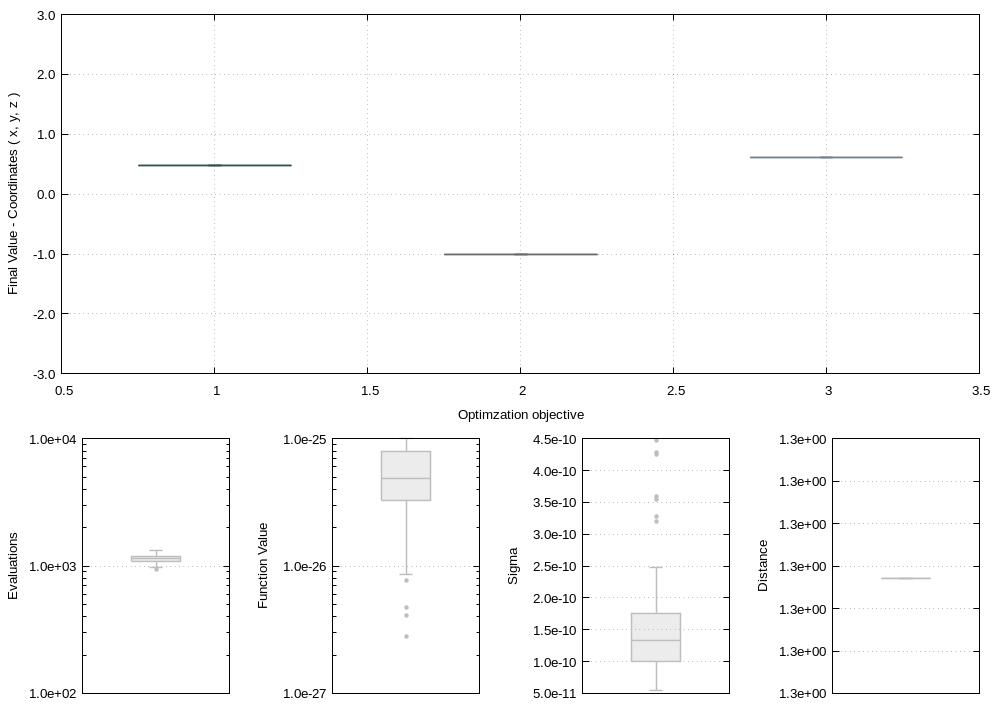
\includegraphics[width=\textwidth]{img/calibration/calibration_ant0-boxes.png}
                 \caption{lorem}
                 \label{fig:Final_Calibration_Ant0_ES-boxes}
         \end{subfigure}
%
\qquad         
%
         \begin{subfigure}[h]{0.4\textwidth}
                 \centering
                 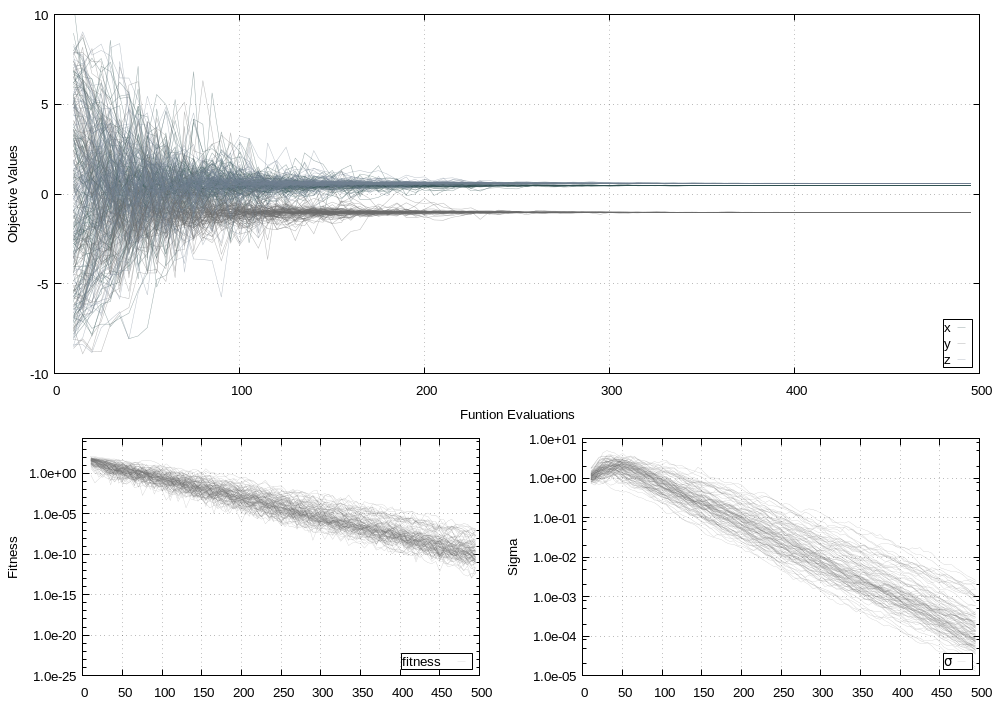
\includegraphics[width=\textwidth]{img/calibration/calibration_ant0-lines.png}
                 \caption{lorem}
                 \label{fig:Final_Calibration_Ant0_ES-Lines}
         \end{subfigure}
%
\\
%
         \begin{subfigure}[h]{0.4\textwidth}
                 \centering
                 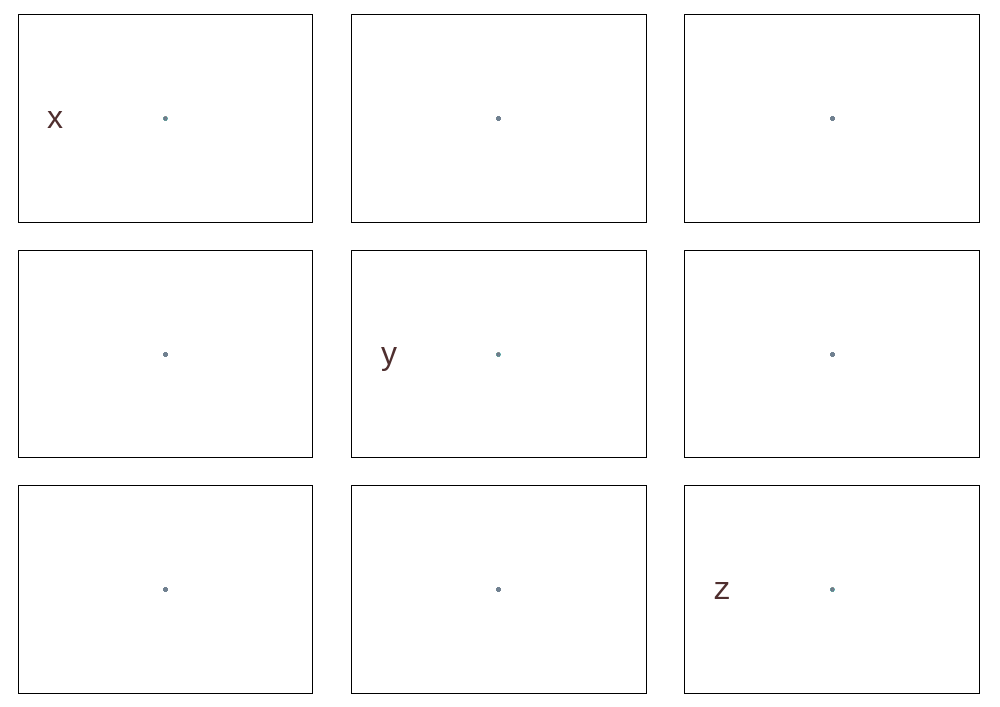
\includegraphics[width=\textwidth]{img/calibration/calibration_ant0-scatter.png}
                 \caption{lorem}
                 \label{fig:Final_Calibration_Ant0_ES-Scatter}
         \end{subfigure}
%
         \caption{Ergebnisse der evolutionären Kalibrierung. Es wurden insgesamt $100$ Durchläufe des Algorithmus erstellt. In (a) wird der Endwert einer jeden Lösung gezeigt, Dabei werden oberes und unteres Quartil sowie der Mittelwert mit Hilfe von Boxen dargestellt; (b) zeigt den Verlauf der drei Objektvariablen aller Durchläufe sowie die Entwicklung der Fitness und das mittlere Sigma. Das Abbruchkriterium war eine Fitness von $\leq 10^{-25}$. Die Fähnchen der Boxen, stellen die maximal- bzw. minimal-Werte dar. Die Große enthält der obere und untere Quartil der Daten, der Strich in der Box zeigt den Mittelwert aller Lösungen. }
         \label{fig::Final_Calibration_Ant0}
\end{figure}
%
\begin{figure}[h]
         \centering
         \begin{subfigure}[h]{0.4\textwidth}
                 \centering
                 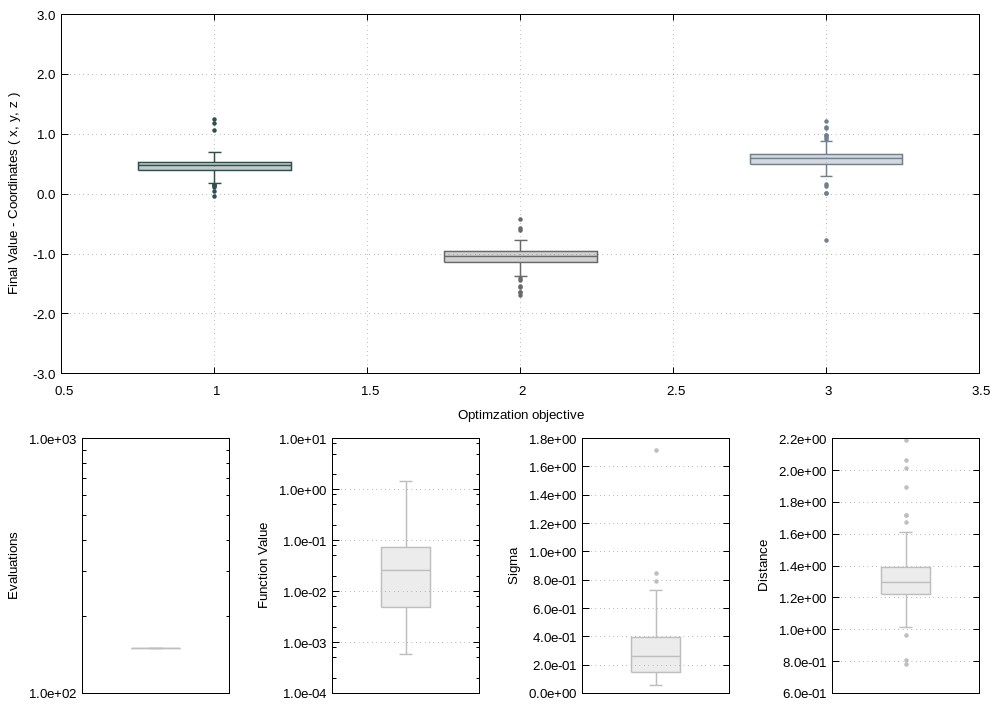
\includegraphics[width=\textwidth]{img/calibration/aborted_calibration_ant0-boxes.png}
                 \caption{Statistisch verteilte Endwerte für die Koordinaten der Kalibrierung. Die Werte für x,y, und z haben noch nicht ihren Endwert erreicht.}
                 \label{fig:abortedFinal_Calibration_Ant0_ES-boxes}
         \end{subfigure}
%
\qquad         
%
         \begin{subfigure}[h]{0.4\textwidth}
                 \centering
                 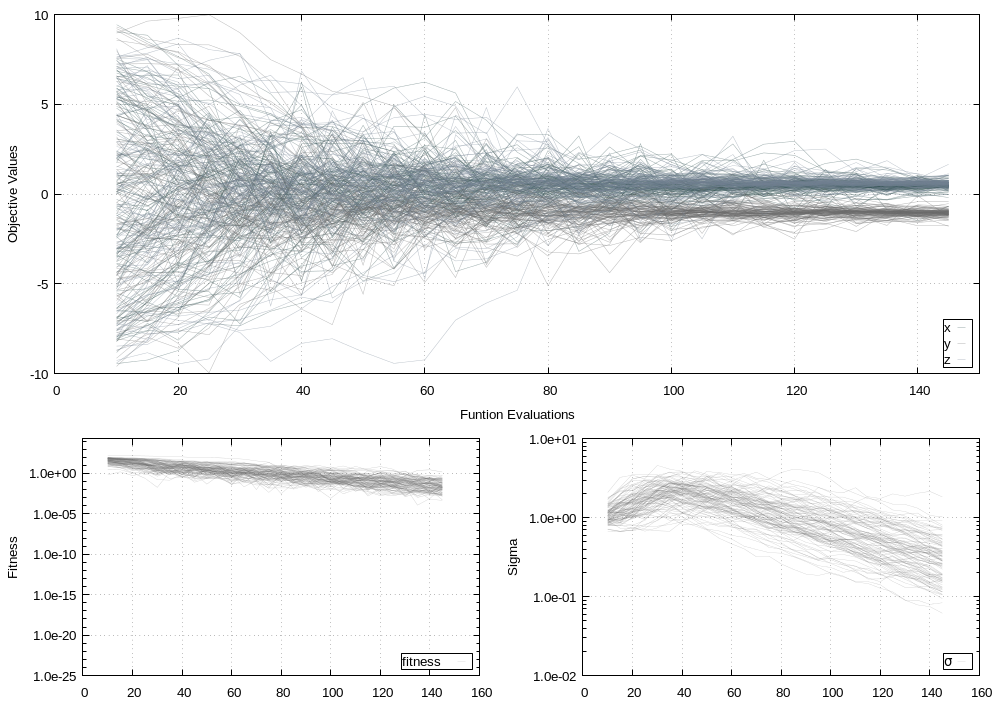
\includegraphics[width=\textwidth]{img/calibration/aborted_calibration_ant0-lines.png}
                 \caption{lorem}
                 \label{fig:abortedFinal_Calibration_Ant0_ES-Lines}
         \end{subfigure}
%
\\
%
         \begin{subfigure}[h]{0.4\textwidth}
                 \centering
                 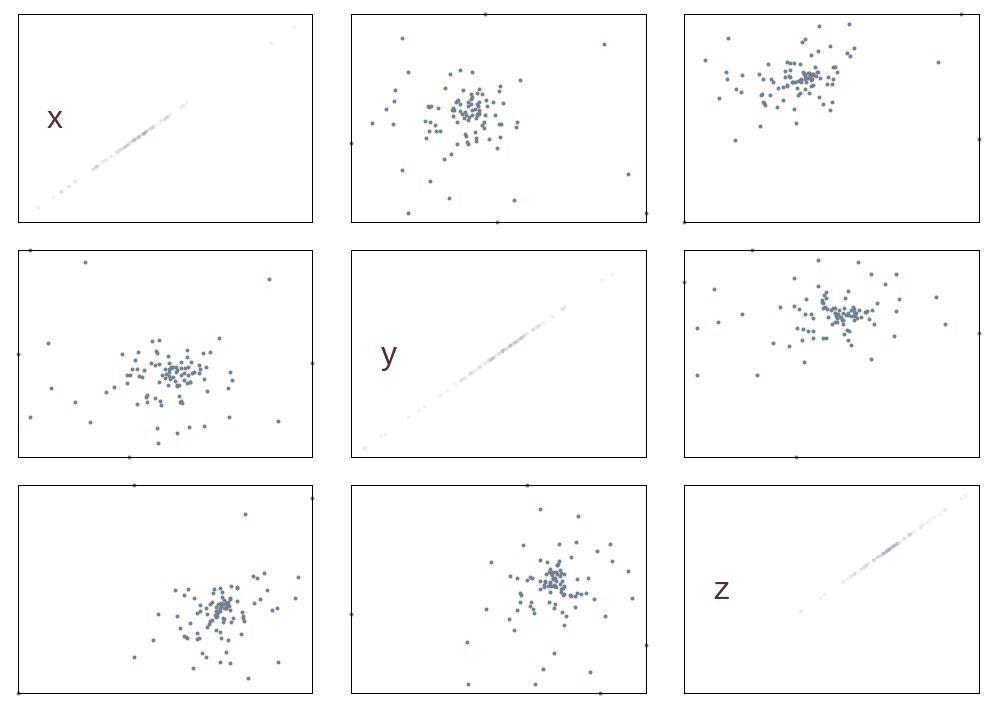
\includegraphics[width=\textwidth]{img/calibration/aborted_calibration_ant0-scatter.png}
                 \caption{lorem}
                 \label{fig:abortedFinal_Calibration_Ant0_ES-Scatter}
         \end{subfigure}
%
         \caption{Analog zu der Abbildung \ref{fig::Final_Calibration_Ant0} zeigen die Plots die gleichen Darstellungen. Diese zeigt, wie sich eine Statistische Verteilung in den Plots Manifestieren würde. Um das zu demonstrieren wurde das Abbruchkriterium auf lediglich $150$ Evaluationen der Zielfunktion eingestellt. Zu diesem Zeitpunkt können die Objektvariablen bereits einen passablen Wert erreicht haben oder noch abweichende Werte aufweisen (vgl. \ref{fig:Final_Calibration_Ant0_ES-Lines}).}
         \label{fig::abortedFinal_Calibration_Ant0_ES}
\end{figure}
%
\begin{figure}[h]
         \centering
         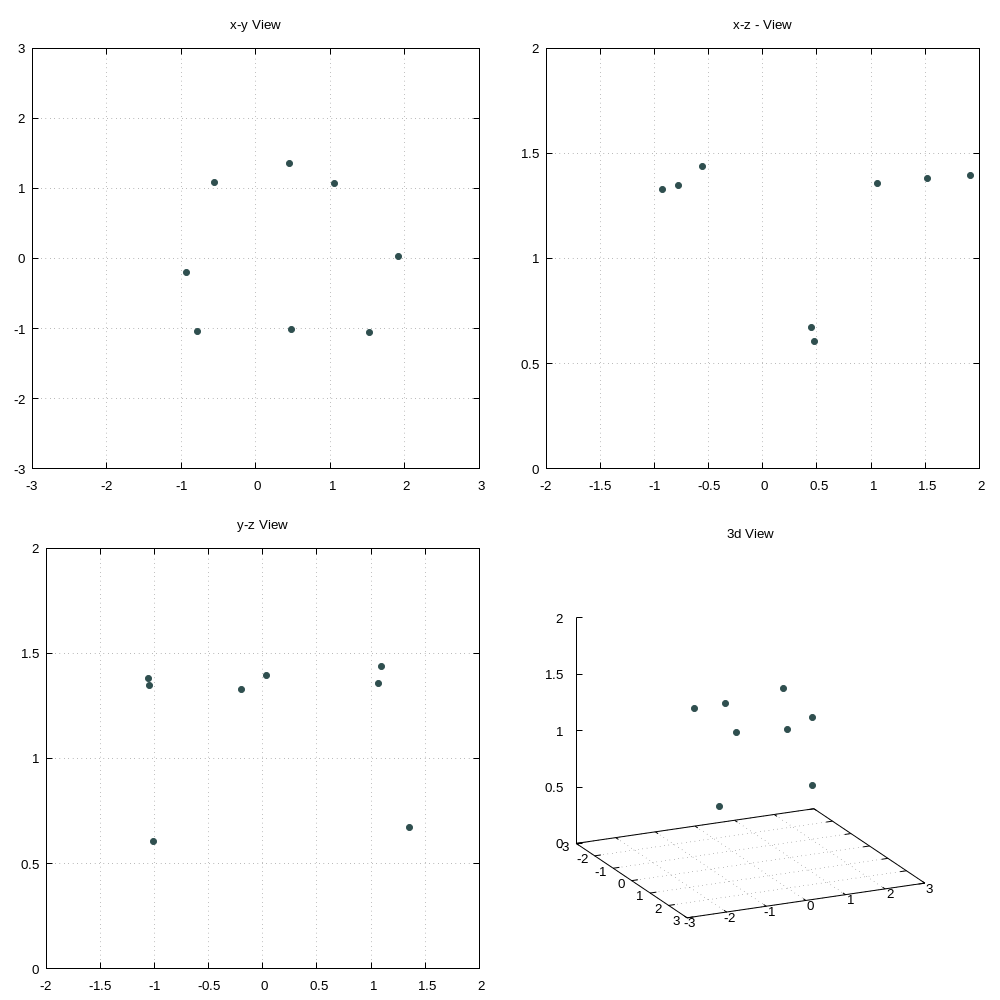
\includegraphics[width=0.4\textwidth]{img/calibration/calibration_results.png}
         \caption{Das visualisierte Endergebnis der Kalibrierung.}
         \label{fig:3dplot_coordinates}
%
\end{figure}

\begin{figure}[h]
         \centering
         \begin{subfigure}[h]{0.4\textwidth}
                 \centering
                 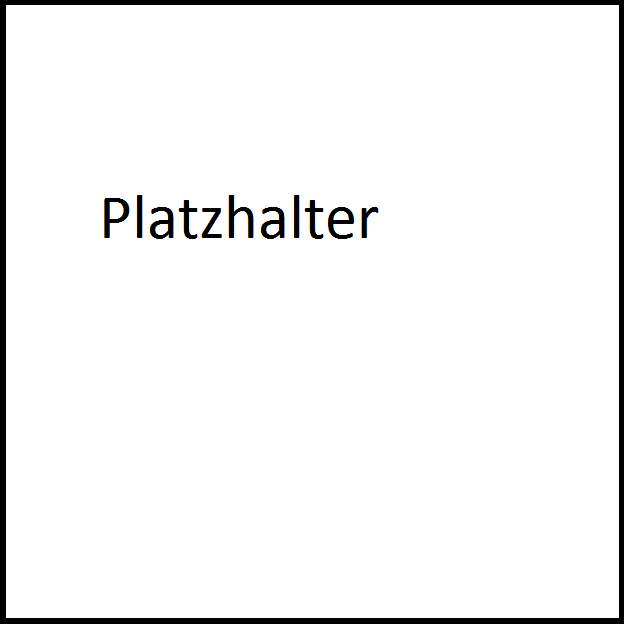
\includegraphics[width=\textwidth]{img/00_placeholder-sqare.png}
                 \caption{Laser Entfernungsmesser der Fa. Bosch}
                 \label{fig:laser_meter}
         \end{subfigure}
%
\qquad         
%
         \begin{subfigure}[h]{0.4\textwidth}
                 \centering
                 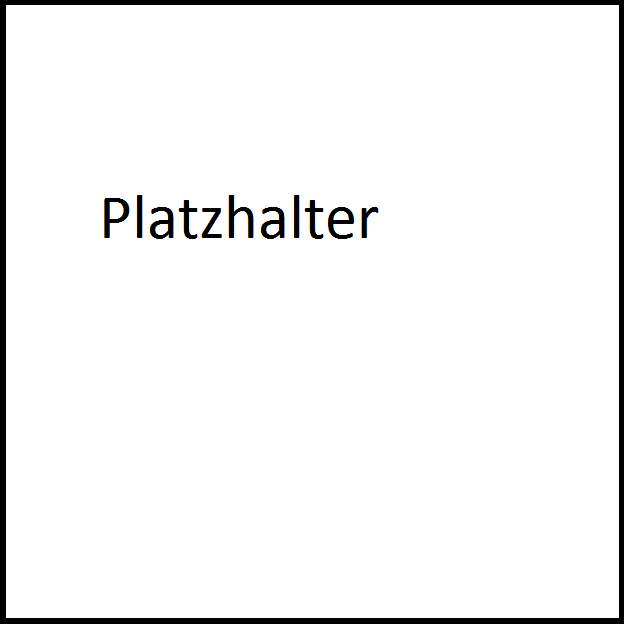
\includegraphics[width=\textwidth]{img/00_placeholder-sqare.png}
                 \caption{Kalibrierstück, verwendet zum Einmessen des Antennenaufbaus}
                 \label{fig:calib_piece}
         \end{subfigure}
         \caption{Werkzeuge die bei der Kalibrierung verwendet werden.}
         \label{fig:Calibration_Tools}
\end{figure}
 